%% Placeholder for discussion of duality

%Below are notes for Nov 20
In optimization theory, duality or the duality principle is the principle that optimization problems may be viewed from either of two perspectives, that is, the primal problem or the dual problem.

Let's consider the primal problem formulated as follows,
\begin{align*}
\min \quad&F_0(x) \\
s.t. \quad&F_i(x)\leq 0, i = 1,...,m\\
&h_i(x)= 0, i = 1,...,p
\end{align*}
Note that we do not have any assumptions of convexity here.

So the feasible set for this problem is
$$D = (\cap^m_{i=1}\text{dom}\ F_i)\cap(\cap^p_{i=1}\text{dom}\ h_i)$$ 
and the optimal value is $p^*$, optimal variable is $x^*$.

\begin{definition}[The Lagrangian Function]
	We define the Lagrangian function as follows,
	$$L(x,\lambda,\nu) := F_0(x) + \sum^m_{i=1}\lambda_i F_i(x) + \sum^p_{i=1}\nu h_i(x)$$
	where
	$$\lambda =
	\begin{bmatrix}
		\lambda_1\\
		\lambda_2\\
		\vdots\\
		\lambda_m
	\end{bmatrix},\
	\nu = 
	\begin{bmatrix}
		\nu_1\\
		\nu_2\\
		\vdots\\
		\nu_p
	\end{bmatrix}$$

The pairs $(\lambda, \nu)$ are called the "Lagrange multipliers" or "dual variables", and the domain for the Lagrangian function is given by 
$$\text{dom}\ L = D\times \reals^m \times \reals^p$$
\end{definition}

\begin{definition}[The "dual" function]
	The dual function $g(\cdot, \cdot)$ is defined as 
	\begin{equation*}
	g(\lambda, \nu) = \min_{x\in D}\quad L(x,\lambda,\nu)
	\end{equation*}
	
	Note: removes dependence on $x$.
\end{definition}


\begin{definition} The dual optimization problem is formulated as
	\begin{align*}
	\max_{\lambda, \nu} \quad&g(\lambda, \nu) \\
	s.t. \quad&\lambda \geq 0
	\end{align*}

Note: $\nu_i$ are unconstrained, and we denote the optimal value as $d^*$, optimal dual variables as $\lambda^*$ and $\nu^*$.
\end{definition}


\vspace{0.3cm}
Duality Theory: For most convex optimization problem, $d^* = p^*$.\\


\begin{align*}
\min \quad&F_0(x) \\
s.t. \quad&F_i(x)\leq 0, \quad i = 1,...,m \\
&h_i(x)= 0, \quad i = 1,...,p
\end{align*}

\begin{equation*}
L(x,\lambda,\nu) = F_0(x) + \sum^m_{i=1}\lambda_i F_i(x) + \sum^p_{i=1}\nu_i h_i(x)
\end{equation*}

Dual Function:

\begin{equation*}
g(\lambda, \nu) = \min_{x\in D}\quad L(x,\lambda,\nu) 
\end{equation*}


\begin{align*}
\max \quad&g(\lambda, \nu) \\
s.t. \quad&\lambda \geq 0
\end{align*}
\begin{enumerate}

\item $g(\lambda, \nu)$ is concave in $(\lambda, \nu)$ for all $F_0,...,F_m$, $h_0,...,h_p$.

\begin{proof}
Recall that
$$g(\lambda, \nu) =\min_{x\in D}[F_0(x) + \sum^m_{i=1}\lambda_iF_i(x) + \sum^p_{i=1}\nu_ih_i(x) ]$$

First, notice that Lagrange function is an affine function in $(\lambda, \nu)$ so it is concave(of course it is convex at the same time). Secondly, note that the dual function is a pointwise infimum of a family of affine functions in $(\lambda, \nu)$, and thus $g(\lambda, \nu)$ is concave.
\end{proof}

\item For any primal feasible $x$ (i.e., $F_i(x)\leq 0, \forall i = [m]$, $h_i(x)= 0,\forall i = [p]$ and dual feasible $(\lambda, \nu)$ (i.e., $\lambda \geq 0$), we have
	$$g(\lambda, \nu)\leq F_0(x)$$
    for any tuple $(x, \lambda, \nu) \in \mathcal{C}\times \reals^m_+\times \reals^p$, where $\mathcal{C}$ is the feasible set of the primal problem (contains all feasible $x$).

\begin{proof}
	Notice that, we have
	\begin{align*}
	F_0(x) &\geq F_0(x) + \sum^m_{i=1}\lambda_iF_i(x) + \sum^p_{i=1}\nu_ih_i(x)\\
	&\geq \min_{x\in D} [F_0(x) + \sum^m_{i=1}\lambda_iF_i(x) + \sum^p_{i=1}\nu_ih_i(x)] \\
	&= g(\lambda, \nu)
	\end{align*}
	where the first summation on r.h.s is negative due to $\lambda_i\geq 0$ and $F_i(x)\leq 0$, and the second summation equals to zero due to $h_i(x)=0$. 
	
	Thus the desired result can be obtained by the definition of $\min$ function and dual function.
\end{proof}

The point of greatest interest is $x^*$, where $p^* = F_0(x^*)$.

Plug in to the above inequality, for all dual feasible $(\lambda, \nu)$ (i.e., for $\lambda \geq 0$), we have
\begin{equation*}
p^* = F_0(x^*) \geq g(\lambda, \nu)
\end{equation*}

Optimize over $(\lambda, \nu)$ where $\lambda \geq 0$ in order to maintain dual feasibility, we can get the greatest lower bound,
\begin{equation*}
p^* = F_0(x^*) \geq g(\lambda^*, \nu^*) = d^*
\end{equation*}

That is, we have the so called \textbf{weak duality}, $p^*\geq d^*$. 

Furthermore, we refer to the difference $p^* - d^*$ as the \textbf{optimal duality gap}.


\item For convex primal optimization problems, (i.e., $F_i(x)$ are convex and $h_i(x)$ are affine) and under certain conditions called "constraint qualification"(i.e. not all constraint sets allowed), then the \textbf{strong duality} holds, i.e.,
 $$p^* = d^*$$
 and thus optimal duality gap is zero.

There are many types of constraint qualification, and we will introduce a simple one called Slater's condition in the next section.

\end{enumerate}

%Above are notes for Nov 20

% Below are notes for Nov 25
\subsection{Slater Conditions}

\begin{definition}[Slater conditions]
Consider a primal problem with a set of constraints $F_i(x)\leq 0$, $i = [m]$ and $Ax = b$, it is said to be satisfied the Slater's conditions if there exists an $x\in\text{relint}\ D$ such that

\begin{enumerate}
	\item $F_i(x) < 0,\ \forall i = [m]$
	
	\item $Ax = b$
\end{enumerate}

Furthermore, if some of the inequality contraints are defined by affine functions, this conditions can be weaken a bit. Suppose $F_i$ are affine for $i=1,\cdots, k$, $k<m$, then the Slater conditions requires that there exists an $x\in\text{relint}\ D$ such that
\begin{enumerate}
	\item $F_i(x) \geq 0,\ \forall i = 1,\cdots, k$
	\item $F_i(x) < 0,\ \forall i = k+1,\cdots,m$.
	\item $Ax = b$
\end{enumerate}

\end{definition}

\begin{example}
	Convex problem that doesn't satisfy Slater's:
	\begin{align*}
	\begin{bmatrix}
	(x_1-1) & x_2
	\end{bmatrix}\begin{bmatrix}
	1&0\\
	0&1
	\end{bmatrix}\begin{bmatrix}
	x_1 - 1\\
	x_2
	\end{bmatrix}\leq 1\\
	\begin{bmatrix}
	(x_1+2) & x_2
	\end{bmatrix}\begin{bmatrix}
	1&0\\
	0&0
	\end{bmatrix}\begin{bmatrix}
	x_1 + 2\\
	x_2
	\end{bmatrix}\leq y
	\end{align*}
\end{example}

Feasible set is $(x_1, x_2) = \{(0,0) \}$

\begin{marginfigure}
\centering
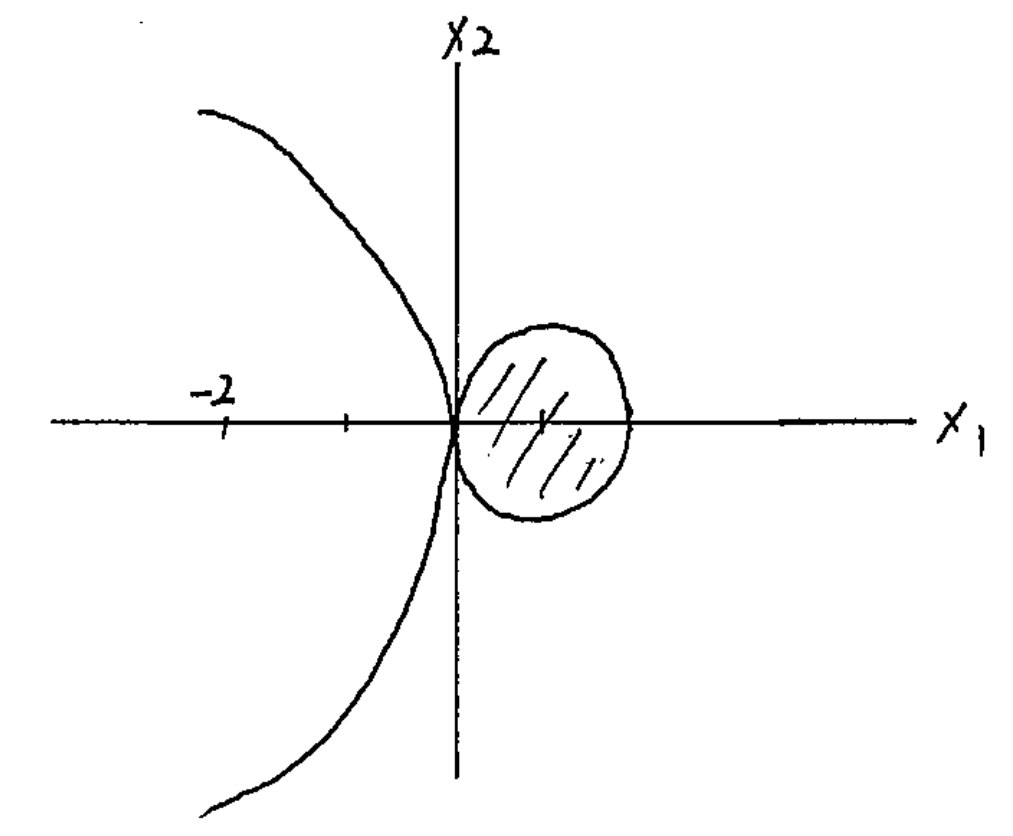
\includegraphics[width=1.8in,height=1.8in]{figures/ch10/figure1125_1.png}
%\caption{This is an inserted JPG graphic} 
%\label{fig:graph} 
\end{marginfigure}

\begin{theorem}
	If the primal optimization problem is convex and satisfies Slater's conditions, then $p^* = d^*$, the strong duality holds.
\end{theorem}

Sketch proof for $m = 1$ (i.e. 1 inequality constraint $p = 0$).

Primal problem:

\begin{align*}
\min \quad & F_0(x)\\
s.t. \quad & F_1(x) \leq 0
\end{align*}

$\Rightarrow$optimal solution $p^*$.

Lagrange function: $L(x, \lambda) = F_0(x) + \lambda F_1(x)$

Dual function: $g(\lambda) = \min_{x\in D} L(x,\lambda) = \min_x{F_0(x) + \lambda F_1(x)}$

Dual optimal: 

\begin{align*}
\max \quad & g(\lambda)\\
s.t. \quad & \lambda  \geq 0
\end{align*}

$\Rightarrow$ dual optimal is $d^*$.

To start, define:

\begin{align*}
G &= \{(F_1(x), F_0(x)) \vert x\in D = domF_1\cap domF_0 \}\\
&= \cup_{x\in D}\{(F_1(x), F_0(x)) \}
\end{align*}

\begin{marginfigure}
\centering
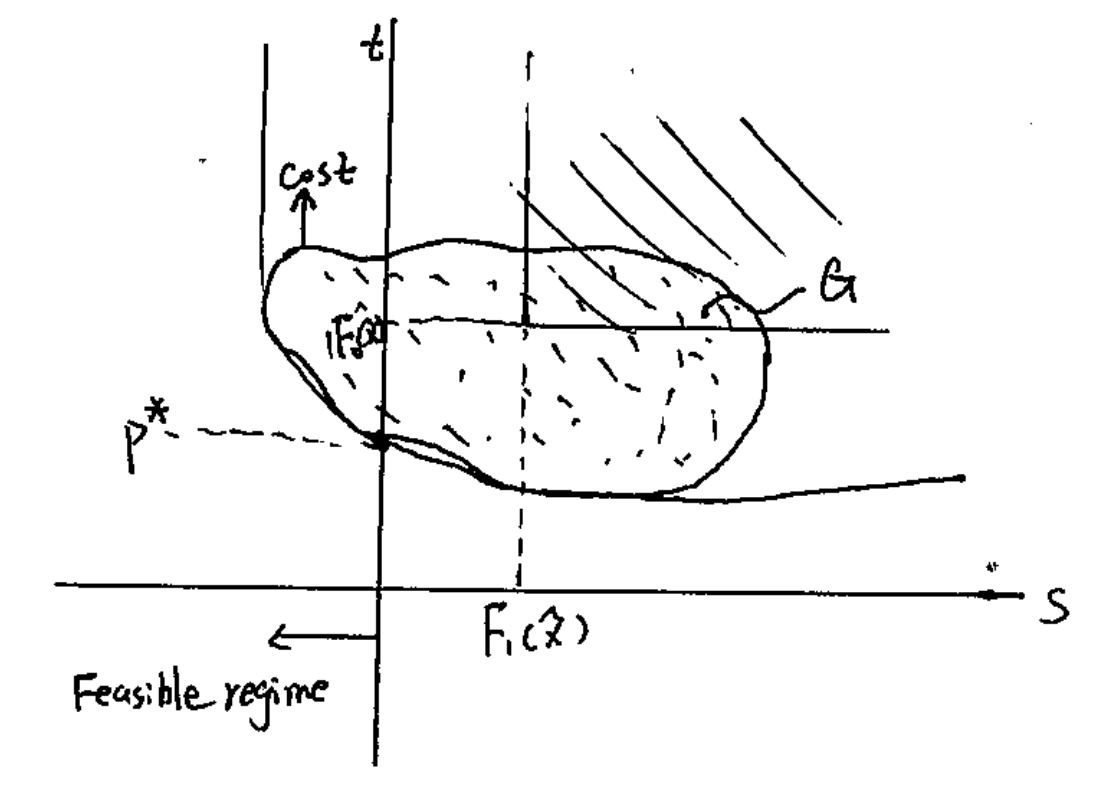
\includegraphics[width=1.8in,height=1.8in]{figures/ch10/figure1125_2.png}
%\caption{This is an inserted JPG graphic} 
%\label{fig:graph} 
\end{marginfigure}

We can let:

\begin{align*}
\mathcal{A} &= G + \reals_+ \times \reals_+\\
&= \{(s,t) \vert F_1(x)\leq s, F_0(x)\leq t, x\in D \}\\
&= \cup_{x\in D}\{(s,t)\vert F_1(x)\leq s, F_0(x)\leq t \}
\end{align*}

Observations: 

\begin{itemize}
	\item $F$ contains all information about primal problem.
	
	\item $\mathcal{A}$ contains all points "above" \& to "right" of each point in $G$.
	
	$\rightarrow$ each such point(above and to right) is less interesting than the point in $G$.
	
	(1) Perhaps higher cost
	
	(2) Perhaps more resources
\end{itemize}

The boundary of $\mathcal{A}$ is specified by the function:
\begin{align*}
p(x) = &\min \quad F_0(x)\\
&s.t. \quad F_i(x) \leq u
\end{align*}
($p$ is the boundary, $\mathcal{A}$ lies above the boundary)

\begin{enumerate}
	\item $p^* = p(0)$
	
	\item $p$ is non-increasing in $\mathcal{U}$
	
	\item $p$ is convex in $\mathcal{U}$
	
	\item $\mathcal{A} = epi\, p$
\end{enumerate}
Proof of (1): 
\begin{proof}
	As $u$ gets larger, feasible set of the $p(u)$ optimization gets larger so objective cannot increase $\rightarrow$ therefore non-increasing.
\end{proof}

Proof of (2):

\begin{proof}
	Convexity of
	\begin{align*}
	p(x) = &\min \quad F_0(x)\\
	&s.t. \quad F_i(x) \leq u
	\end{align*}
	
	Need to show $\forall u_1, u_2\in domp$, $\forall \lambda\in [0,1]$:
	
	\begin{equation*}
	p(\lambda u_1 + (1-\lambda)u_2) \leq \lambda  p(u_1) + (1-\lambda)p(u_2)
	\end{equation*}
	
	Let
	
	\begin{align*}
	x_i = &arg \min \quad F_0(x)\\
	&s.t. \quad F_i(x) \leq u_i
	\end{align*}
	
	i.e. $F_0(x_1) = p(u_1)\& F_0(x_2) =p(u_2)$
	
	Let $\tilde{x} = \lambda x_1 + (1-\lambda)x_2$ $\leftarrow$ $x_1\in domF_1\cap domF_0\cap \{x\vert F_1(x)\leq u_1 \}$, $x_2\in domF_1\cap domF_0\cap \{x\vert F_2(x)\leq u_2 \}$($x_1$, $x_2$ from different sets)
	
	\begin{align*}
	F_1(\tilde{x}) &= F_1(\lambda x_1 + (1-\lambda)x_2)\quad (\text{Since } F_1\text{ is convex}, \tilde{x}\in domF_1)\\
	&\leq \lambda F_1(x_1) + (1-\lambda)F_1(x_2)\quad (\text{Since } F_1 \text{ is convex})\\
	&\leq \lambda u_1 + (1-\lambda)u_2 \quad (\text{Since } F_i(x_i) \leq u_i)
	\end{align*}
	
	Hence 
	
	\begin{equation*}
	\tilde{x} \in domF_1 \cup domF_0 \cup \{x\vert F_1(x)\leq \lambda u_1 + (1-\lambda)u_2 \}
	\end{equation*}
	
	
	That is: $\tilde{x}$ is a feasible point for opt problem $p(\lambda u_1+(1-\lambda)u_2)$	
\end{proof}

Think about tradeoff between $F_1(x)$ and $F_0(x)$ in a slightly different way:


\begin{align*}
\min_{(s,t)} \quad&\lambda s + t\\
\text{where} \quad&(s,t) \in \mathcal{A}
\end{align*}

$\Leftrightarrow$

\begin{align*}
\min \quad&\begin{bmatrix}
\lambda &1 
\end{bmatrix}\begin{bmatrix}
s\\
t
\end{bmatrix}\\
\text{where} \quad &(s,t) \in \mathcal{A}
\end{align*}

\begin{marginfigure}
\centering
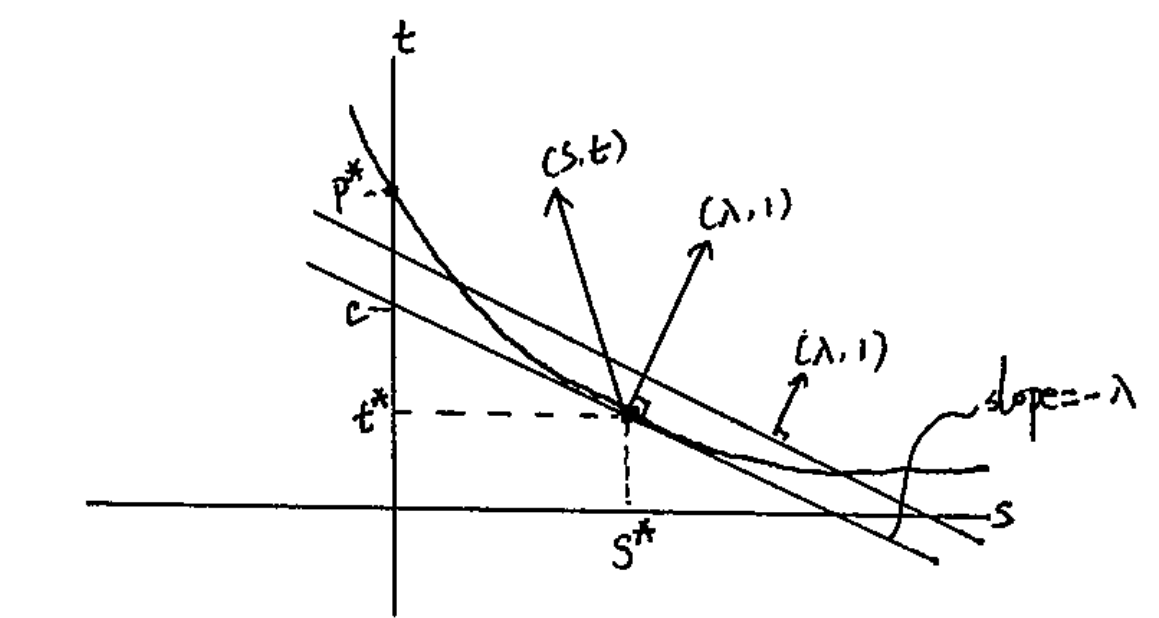
\includegraphics[width=1.8in,height=1.8in]{figures/ch10/figure1125_3.png}
%\caption{This is an inserted JPG graphic} 
%\label{fig:graph} 
\end{marginfigure}

For a given $\lambda$ optimum is attained by some point $(s^*, t^*)$ on boundary of $\mathcal{A}$. Point on boundary is a function of $\lambda$ $(s^*(\lambda), t^*(\lambda)) = (F_1(x^*(\lambda)), F_0(x^*(\lambda)))$. 

Consider any point $(s,t)\in \mathcal{A}$:

\begin{align*}
\begin{bmatrix}
\lambda &1
\end{bmatrix}\begin{bmatrix}
F_1(x^*(\lambda))\\
F_0(x^*(\lambda))
\end{bmatrix}&\leq \begin{bmatrix}
\lambda &1
\end{bmatrix}\begin{bmatrix}
s\\
t
\end{bmatrix}\quad  (*)\\
0&\leq \begin{bmatrix}
\lambda & 1
\end{bmatrix}(\begin{bmatrix}
s\\
t
\end{bmatrix} - \begin{bmatrix}
F_1(x^*(\lambda))\\
F_0(x^*(\lambda))
\end{bmatrix})
\end{align*}

\begin{enumerate}
	\item This optimization yields a tangent plane "supporting hyperplane"
	
	\item In this $2-D$ picture, supporting hyper-plane is a line, change $"\leq"$ in $(*)$ to get line 
	
	\begin{equation*}
	c =\lambda s + t
	\end{equation*} of $(*)$.
	
	re-arrange $t = c - \lambda s$.
\end{enumerate}


This is the problem we just talked about:

\begin{align*}
\min_{(s,t)\in \mathcal{A}} \quad \lambda s + t &= \lambda s^* + t^*\\
&= \lambda F_1(x^*(\lambda)) + F_0(x^*(\lambda))\\
&= \min_{x\in D} \quad[\lambda F_1(x) + F_0(x)]\\
&= g(\lambda) 
\end{align*} the "Dual Function"

Put together pieces:






\begin{itemize}
	\item The dual function $g(x)$ specifies the $y-$intercept of the tangent line of slope $-\lambda$.
	
	\item Last time proves $g(\lambda)$ is a lower bound on $p^*$ as long as $\lambda$ are dual-feasible ($\lambda \geq 0$)
	
	\item The $y-$intercept is a lower bound on $p^*$
\end{itemize}

Get best lower bound by maximizing $g(\lambda)$ over $\lambda > 0$, solve:

\begin{align*}
\max \quad &g(\lambda)\\
s.t. &\lambda \geq 0
\end{align*}




% Above are notes for Nov 25



% Below are notes for Nov 27

\begin{align*}
\max \quad &F_0(x)\\
s.t. \quad&F_1(x) \leq 0\\
\\
L(x,\lambda) &= F_0(x) + \lambda F_1(x)\\
g(\lambda) &= \min_{x\in D} L(x,\lambda)\\
d^* &= \max \quad g(\lambda)\quad s.t.\quad \lambda \geq 0 
\end{align*}

\begin{equation*}
\mathcal{A} =\{(s,t)\vert F_1(x)\leq s, F_0(x)\leq t, x\in D \}
\end{equation*}


\begin{marginfigure}
\centering
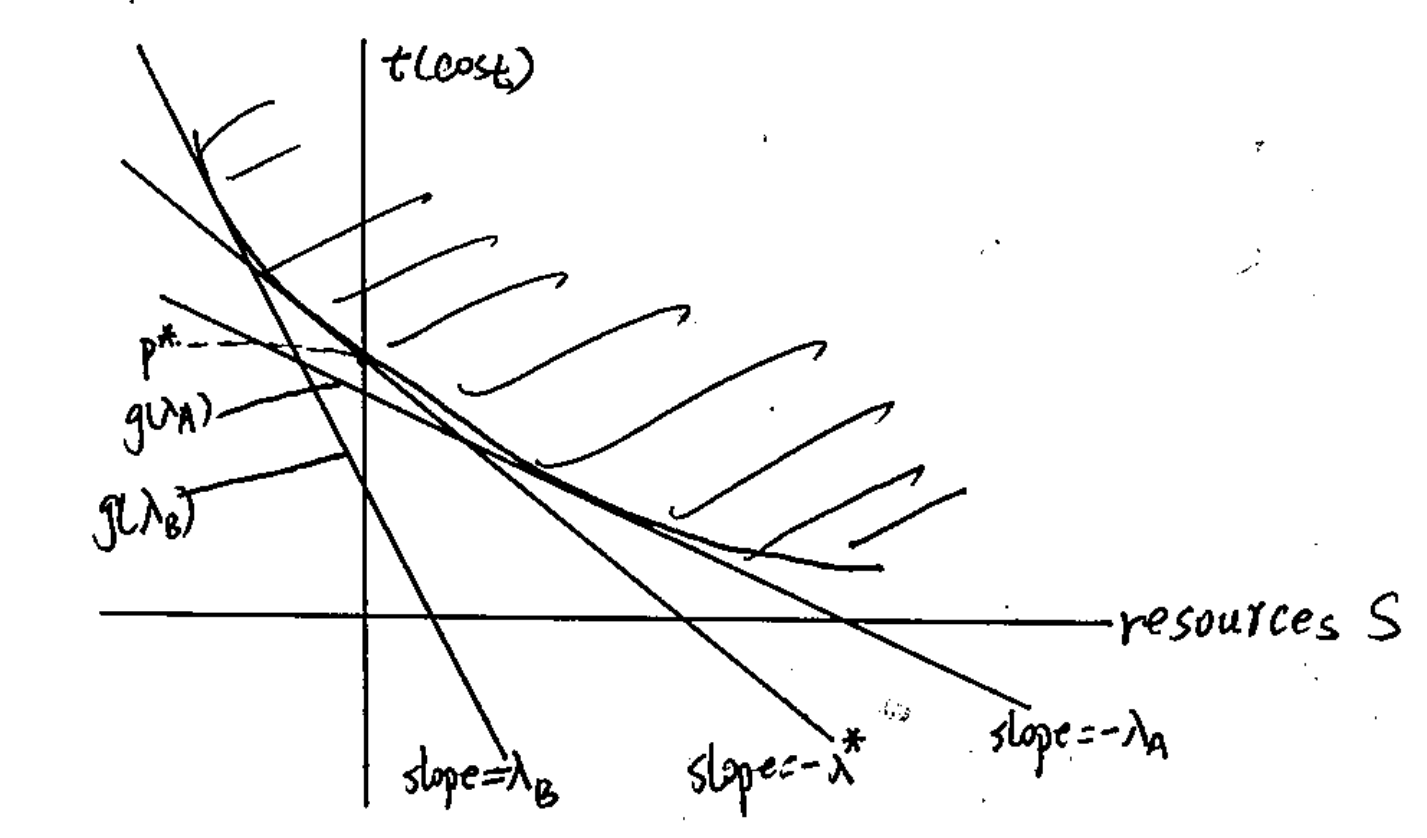
\includegraphics[width=1.8in,height=1.8in]{figures/ch10/figure1127_1.png}
%\caption{This is an inserted JPG graphic} 
%\label{fig:graph} 
\end{marginfigure}



\subsection{"Pricing" Interpretation}


\begin{align*}
\min \quad & F_0(x)\\
s.t.\quad & F_i(x) \leq 0,\quad i = 1,...,m\\
& h_i(x) = 0,\quad i = 1,...,p
\end{align*}

$\rightarrow$ reformulate as an unconstrained problem by introducing $I\& \tilde{I}$


\begin{equation}
\label{eq6}
I(x)=\left\{
\begin{aligned}
0 & , & x\leq 0 \\
\infty & , & x>0
\end{aligned}
\right.
\end{equation}

\begin{marginfigure}
\centering
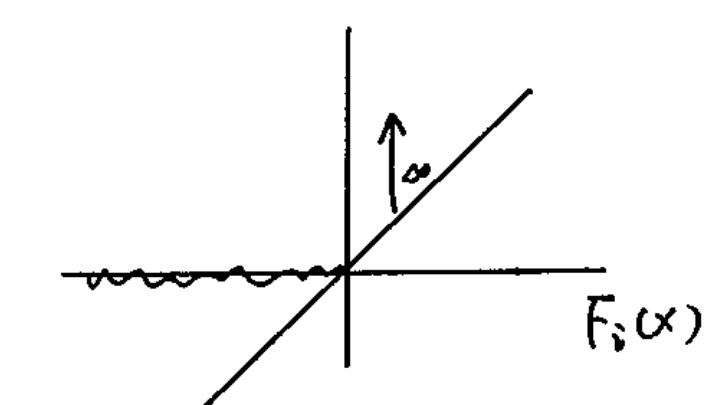
\includegraphics[width=1.8in,height=1.8in]{figures/ch10/figure1127_2.png}
%\caption{This is an inserted JPG graphic} 
%\label{fig:graph} 
\end{marginfigure}

\begin{equation}
\label{eq6}
\tilde{I}(x)=\left\{
\begin{aligned}
0 & , & x= 0 \\
\infty & , & \text{else}
\end{aligned}
\right.
\end{equation}


\begin{marginfigure}
\centering
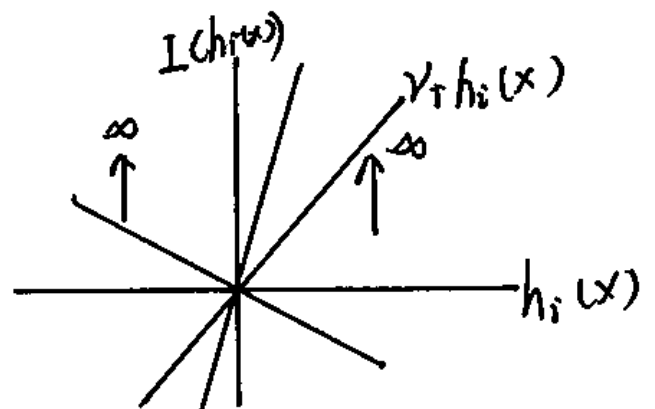
\includegraphics[width=1.8in,height=1.8in]{figures/ch10/figure1127_3.png}
%\caption{This is an inserted JPG graphic} 
%\label{fig:graph} 
\end{marginfigure}


\begin{equation*}
\min_x\quad F_0(x) + \sum^m_{i=1}I(F_i(x)) + \sum^p_{i=1}\tilde{I}(h_i(x)) \qquad (*)
\end{equation*}

$\Rightarrow$ Same problem but with "hard" penalties

$I$ and $\tilde{I}$

\begin{equation*}
F_0(x) + \sum^m_{i=1}\lambda_i F_i(x) + \sum^p_{i=1}\nu_i h_i(x)
\end{equation*}

$\lambda_i$ = "price" for violating constraint $F_i$, $\mu_i$ = "price" for violating constraint $h_i$.

If strong duality holds:

\begin{align*}
(*) &= \max_{\lambda, \nu, \lambda \geq 0}\quad [\min_x\quad F_0(x) + \sum^m_{i=1}\lambda_iF_i(x) + \sum^p_{i=1}\nu_ih_i(x)]\\
&= \max_{\lambda, \nu}\quad g(\lambda, \nu)\qquad \lambda \geq 0
\end{align*}

Adjust prices $\lambda, \nu$ so that the solution to relaxed problem matrices the solution to primal
\subsection{Sensitivity Analysis}

\begin{marginfigure}
\centering
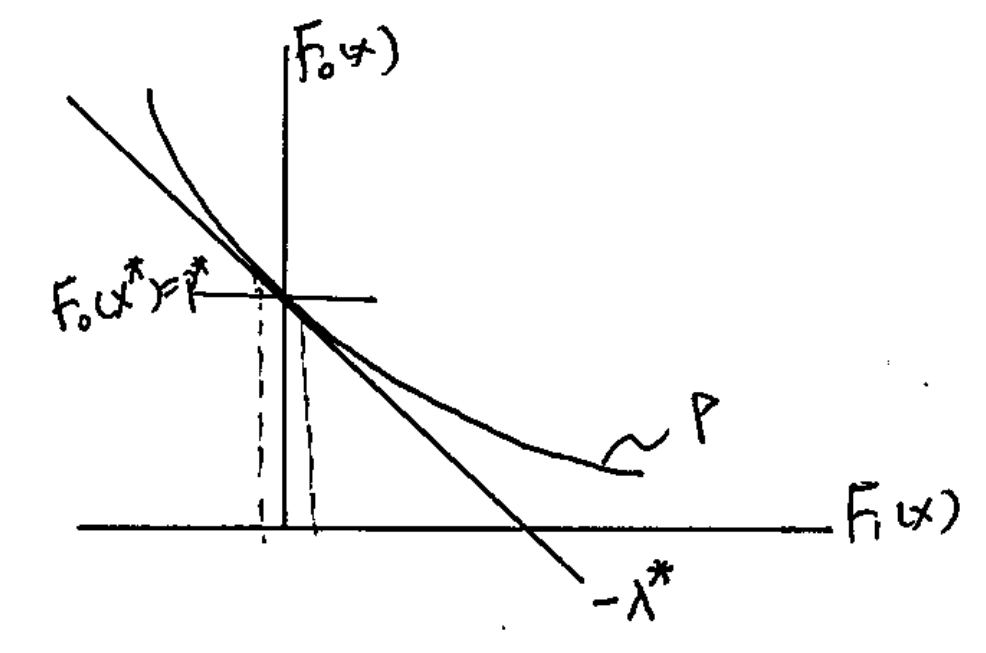
\includegraphics[width=1.8in,height=1.8in]{figures/ch10/figure1127_4.png}
%\caption{This is an inserted JPG graphic} 
%\label{fig:graph} 
\end{marginfigure}

$\rightarrow$ At dual optimum slope of tangent is $-\lambda^*$

$\rightarrow$
 If change constraint by $\epsilon$, optimum value will change by something like $(-\epsilon \lambda^*)$.
 
 
\begin{align*}
p^*(u,v) = \min \quad &F_0(x) \\
s.t.\quad & F_i(x) \leq 0,\quad i = 1,...,m\\
& h_i(x) = 0,\quad i = 1,...,p
\end{align*}




$\rightarrow$ $u_i<0$ "tighten" constraint, $u_i>0$ loosen constraint, $v_i\neq 0$ change set-point.

$\rightarrow$ Same as $p(u)$ in last lecture.

$\rightarrow$ Note $p^*(0,0) = p^*$ optimal value unconstrained problem

$\rightarrow$ relate $p^*(u,v)$ to $p^*(0,0)$\\

\begin{itemize}
	\item Let $(\lambda^*, \nu^*)$ be optimal dual variables for unperturbed problem
	
	\item Consider a convex optimization problem satisfying Slater's $\rightarrow$ strong duality holds
	
	\begin{align*}
	p^*(0,0) &= g(\lambda^*, \nu^*)\\
	&= \min_{x\in D} L(x, \lambda^*, \nu^*)\\
	&\leq F_0(x) + \sum^m_{i=1}\lambda_i^* F_i(x) + \sum^p_{i=1}\nu_i^* h_i(x)\\
	&\leq F_0(x) + \sum^m_{i=1}\lambda_i^* u_i + \sum^p_{i=1}\nu^*_iv_i\\
	&= F_0(x) + (\lambda^*)^Tu+(\nu^*)^Tv
	\end{align*}
\end{itemize}
Focus in on $x\in D$ s.t. $x$ is optimal for perturbed problem

i.e. $F_0(x)=p^*(u,v)$

$\Rightarrow$ $p^*(u,v) \geq p^*(0,0) - (\lambda^*)^Tu - (\nu^*)^Tv$

\begin{enumerate}
	\item E.g. If $\lambda_i >> 0$ and tighten constraint $F_i$ slightly so that $F_i(x)\leq -\epsilon < 0$\\
	
	\begin{equation*}
	p^*(u,v)\geq p^*(0,0) - (\lambda^*)^Tu - (\nu^*)^Tv
	\end{equation*}
	
	\item Note not symmetric in general, big relaxation in constraint doesn't necessary mean big drop in cost.
	
	\item If $p(u,v)$ is differentiable, then have symmetry for small perturbations. 
\end{enumerate}

\subsection{Lagrange Method}
To solve:

\begin{align*}
\min_x\quad F_0(x)\\
s.t. \quad F_i(x) \leq 0,\quad i = 1,...,m
\end{align*}

\begin{enumerate}
	\item First write Lagrangian: $L(x, \lambda) = F_0(x) + \sum^m_{i=1}\lambda_iF_i(x)$
	
	\item Solve for dual $g(\lambda) = \min_{x} L(x, \lambda)$
	
	\item Find $\lambda^* = arg\, \min g(\lambda)$, $s.t. \quad \lambda \geq 0$
	
	\item Recover primal optimal $x^*$ by solving:
	
	\begin{equation*}
	arg\, \min[L(x, \lambda^*) = F_0(x) + \sum^m_{i=1}\lambda_i^*F_i(x)]
	\end{equation*}
\end{enumerate}

\begin{itemize}
	\item Nice approach if problem has nice structure, in particular if easy to solve for $(\lambda^*, \nu^*)$ analytically or numerically. 
	
	\item Even if $(\lambda^*, \nu^*)$ are unique, the $x$ that minimized $L(x, \lambda^*, \nu^*)$ may not be.
\end{itemize}



\begin{example}
	Lagrange Duality for LS problems
	\begin{align*}
	\min_x \quad &\Vert x \Vert_2^2\\
	s.t.\quad &Ax = b
	\end{align*}
	
	"under-determined LS", $x^* = A^T(AA^T)^{-1}b$, $rank(A) = m$
	
	(1) Form Lagrangian $L(x, \nu) = x^Tx + \nu^T(Ax - b)$
	
	
	(2) Evaluate dual
	
	\begin{align*}
	g(\lambda) &= \min_x \quad L(x, \nu)\\
	\frac{\partial}{\partial x} L(x, \nu) &= 2x+A^T\nu = 0\Rightarrow x^*(\nu) = -\frac{1}{2}A^T\nu
	\end{align*}
	
	
	(3) Find
	
	
	\begin{align*}
	\max_{\nu} g(\nu) &= \max_{\nu} L(x^*(\nu)\nu)\\
	&= \max_{\nu}[x^Tx + \nu^T(Ax - b)]\\
	&= \max_{\nu}[\frac{1}{4}\nu^TAA^T\nu + \nu^T(A(-\frac{1}{2}A^T\nu)-b)]\\
	&= \max_{\nu}[\frac{1}{4}\nu^TAA^T\nu - \frac{1}{2}\nu^TAA^T\nu - \nu^Tb]\\
	&= \max_{\nu}[-\frac{1}{4}\nu^TAA^T\nu - \nu^Tb]
	\end{align*}
\end{example}

\begin{align*}
\frac{\partial}{\partial \nu}(-\frac{1}{4}\nu^TAA^T\nu &- \nu^Tb)\\
\frac{1}{4}2AA^T\nu - b &= 0\\
(AA^T)\nu &= -2b\\
\nu^* &= -2(AA^T)^{-1}b
\end{align*}

Substitute into $x^*(\nu)$ to get:

\begin{align*}
x^*(\nu^*) &= -\frac{1}{2}A^T(-2(AA^T)^{-1}b)\\
&= A^T(AA^T)^{-1}b
\end{align*}

Example: Lagrange Duality For LS problems
\begin{align*}
\min_x \quad & \Vert x\Vert^2_2\\
s.t. \quad & Ax = b
\end{align*}

"under-determined LS": $x^* = A^T(AA^T)^{-1}b$.

\begin{equation*}
\frac{1}{4}\nu^TAA^T\nu+\nu^Tb
\end{equation*}

$\Rightarrow$ same as the following $\min_y\quad \Vert\frac{1}{2}A^T\nu + x_0\Vert^2_2$ for any $x_0$ s.t. $Ax_0 = b$.

\begin{align*}
\Vert \frac{1}{2}A^T\nu + x_0\Vert_2^2 &= (\frac{1}{2}A^T\nu+x_0)^T(\frac{1}{2}A^T\nu+x_0)\\
&= \frac{1}{4}\nu^TAA^T\nu + 2\frac{1}{4}\nu^TAx_0 + x_0^Tx_0\\
&= \frac{1}{4}\nu^TAA^T\nu + \nu^Tb+x_0^Tx_0
\end{align*}

Final interpretation:

\begin{align*}
\min \quad & F_0(x)\\
s.t. \quad & F_i(x)\leq 0\quad i = 1,...,m
\end{align*}
Connect to problems with multiple (vector)

Objective $(F_0,F_1,...,F_m)$

One approach is to "scalarize" its objective

\begin{equation*}
F_0(x) + \lambda F_1(x) + \cdots + \lambda_mF_m(x) = F_0(x) + \sum^m_{i=1}\lambda_iF_i(x)
\end{equation*}

% Above are notes for Nov 27


% Below are notes for Dec 2
\subsection{Dual of LPs}

\begin{align*}
\min\quad &c^Tx\\
s.t.\quad &Ax\leq b
\end{align*}

Lagrangian: 

\begin{align*}
L(x,\lambda) &= c^Tx + \sum^m_{i=1}(a_i^Tx-b_i)\\
&= c^Tx+\begin{bmatrix}
\lambda_1&\lambda_2&\cdots&\lambda_m
\end{bmatrix}\begin{bmatrix}
a_i^Tx-b_1\\
\vdots\\
a_m^Tx-b_m
\end{bmatrix} \\
&=c^Tx+\lambda^T(Ax-b)\\
&= -\lambda^Tb-(c^T+\lambda^TA)x
\end{align*}

Dual:

\begin{align*}
g(\lambda) &= \min_x[-\lambda^Tb+(c^T+\lambda^TA)x]\\
&=
\label{eq6}
\left\{
\begin{aligned}
-\lambda^Tb &\quad \text{if} & c^T+\lambda^TA=0 \\
-\infty &\quad \text{if} & c^T+\lambda^TA\neq 0
\end{aligned}
\right.
\end{align*}

Dual optimization:
\begin{align*}
\min\quad &g(\lambda)\\
s.t.\quad &\lambda \geq 0
\end{align*}

$\Rightarrow$
\begin{align*}
\min\quad &g(\lambda)\\
s.t.\quad &\lambda\geq 0\\
&c^T+\lambda^TA=0
\end{align*}

$\Leftrightarrow$

\begin{align*}
\min\quad &-\lambda^Tb\\
s.t.\quad &\lambda\geq 0\\
&c^T+\lambda^TA=0
\end{align*}






\begin{itemize}
	\item Dual of an LP is an LP
	
	\item Maybe not clear from form but have strong duality so $p^*=d^*$.
\end{itemize}

\begin{tabular}{|c|c|c|}
	\hline 
	&Primal & Dual\\
	\hline  
	variables & $n$ & $m$\\
	\hline 
	constant&$m$&$n+m$\\
	\hline 
\end{tabular}


\begin{align*}
\min\quad &b^T\lambda\\
s.t.\quad &-\lambda\leq 0\quad\text{inequality multipliers }z\\
&A^T\lambda = -c\quad \text{equality multipliers }y
\end{align*}

\begin{align*}
L(\lambda,x,y) &= b^T\lambda + z^T(-\lambda)+y^T(A^T\lambda + c)\\
g(z,y) = \min_{\lambda}L(\lambda,z,y) &= \min_{\lambda}y^Tc+[b^T-z^T+y^TA^T]\lambda\\
&=
%\label{eq6}
\left\{
\begin{aligned}
y^Tc &\quad \text{if} &b^T-z^T+y^TA^T=0 \\
-\infty &\quad \text{if} &else
\end{aligned}
\right.
\end{align*}




Dual optimization:
\begin{align*}
\max\quad &g(z,y)\\
s.t.\quad &z \geq 0
\end{align*}
$\Leftrightarrow$


\begin{align*}
\min\quad &y^Tc\\
s.t.\quad &b^T-z^T+y^TA^T=0\\
&z\geq 0
\end{align*}
constants:


\begin{align*}
b^T=y^TA^T &= z^T\\
z&\geq 0
\end{align*}

$\Leftrightarrow$

\begin{equation*}
b^T+y^TA^T \geq 0
\end{equation*}

Thus this problem can also be written as:


\begin{align*}
\max\quad &y^Tc\\
s.t.\quad &b+Ay \geq 0
\end{align*}

$\Leftrightarrow$

\begin{align*}
\max\quad &(-x)^Tc\\
s.t.\quad &b+A(-x) \geq 0
\end{align*}

$\Rightarrow$

\begin{align*}
\max\quad &c^Tx\\
s.t.\quad &Ax \leq b
\end{align*}

% Above are notes for Dec 2
